\documentclass[]{article}
\usepackage{amsmath}
\usepackage{amsfonts}
\usepackage{amsthm}
\usepackage{bm}
\usepackage{fancyvrb}
\usepackage{url}
\usepackage{graphicx}
\usepackage{float}
%opening
\title{APPM 4650 HW 7}
\author{Zane Jakobs}

\begin{document}
	\maketitle
	
	
	\subsection*{2}
	We include the following states (which will be explained below): healthy non-immune ($H_N$), healthy immune ($H_I$), infected dormant ($I_D$), infected active ($I_A$), dead infected ($D_I$), dead uninfected ($D_U$), and zombie ($Z_A$). This model assumes that a person is bitten by a zombie and becomes infected with infection rate $\beta$. The infection then lays dormant for some exponentially-distributed time with parameter $\lambda_I$; at that exponentially-distributed (arrival) time, with probability $\eta$, the infected person recovers and becomes immune to the disease, and with probability $1-\eta$, the infection becomes active. Immunity is not hereditary. A person with an active infection will die within an amount of time randomly sampled from a Gaussian distribution with mean $\mu_D$ and variance $\sigma^2_D$, and become dead and infected. A dead, infected person will, assuming their body is not appropriately destroyed, become a zombie. This process is governed by two exponentially-distributed random variables, one for reanimation (with parameter $\lambda_R$) and one for destruction ($\lambda_D$). This could be simulated by drawing a sample from each R.V., and if the sampled reanimation time is smaller than the sampled destruction time, the body reanimates. A person who dies and is/was not infected will never reanimate. A zombie decays with probability $p_D$ after some Normally-distributed amount of time with mean $\mu_Z$ and variance $\sigma^2_Z$, and becomes equivalent to a dead, uninfected body. Zombies can also be killed by healthy people at constant rate-per-person $\lambda_K$. People also die from non-Zombie causes with death rate $\mu_H$ and are born with birth rate $\lambda_H$ This gives the following equations in the fully-mixed, large-N case:
	\[
	\begin{aligned}
	\dfrac{d H_N(t)}{dt} &= [\lambda_H  - \beta Z_A - \mu_H] H_N(t) + \lambda_H H_I(t)\\
	\dfrac{d I_D(t)}{dt} &= \beta Z_A H_N(t) - \lambda_I I_D(t)\\
	\dfrac{d I_A(t)}{dt} &= \lambda_I [1-\eta] I_D(t)\\
	\dfrac{d H_I(t)}{dt} &= \lambda_I \eta I_D(t)\\
	\dfrac{d D_U(t)}{dt} &= \mu_H [H_N(t) + H_I(t)] + \dfrac{\lambda_D}{\lambda_R + \lambda_D} D_I(t) + p_D Z(t-\mu_Z)\\
	\dfrac{d D_I(t)}{dt} &= I_A(t-\mu_D)\\
	\dfrac{d Z(t)}{dt} &= \dfrac{\lambda_R}{\lambda_R + \lambda_D} D_I(t) - p_D Z(t-\mu_Z) - \lambda_K Z(t)[H_N(t) + H_I(t)]\\ 
	1 &= H_N(t) + I_D(t) + I_A(t) + H_I(t) + D_U(t) + D_I(t) + Z(t) 
	\end{aligned}
	\]
	
	\subsection*{3(a)} We have the ODE
	\[
	\begin{aligned}
	\dfrac{d I_k}{dt} &= -\gamma I_k + (P_k - I_k)\bar{\beta}(\text{number of contacts with infected people})\\
	&= -\gamma I_k + (P_k - I_k)\bar{\beta}\sum\limits_{k'} [P_{k'} P(k'\to k)P(k'\text{ is infected})]\\
	&= -\gamma I_k + (P_k - I_k)\bar{\beta}k\sum\limits_{k'} P_{k'} \left( \dfrac{k'}{n\langle k \rangle} + \dfrac{c}{n k \langle k \rangle} (k' - \langle k \rangle)(k - \langle k \rangle)\right)\dfrac{I_{k'}}{P(k')}\\
	&= -\gamma I_k + (P_k - I_k)\bar{\beta}k\sum\limits_{k'} I_{k'} \left( \dfrac{k'}{n\langle k \rangle} + \dfrac{c}{n k \langle k \rangle} (k' - \langle k \rangle)(k - \langle k \rangle)\right).
	\end{aligned}
	\]
	Dividing by $P_k$, we get
	\[
	\dfrac{d i_k}{dt} = -\gamma i_k + \bar{\beta} (1 - i_k) k \sum\limits_{k'}i_{k'}P_{k'} \left( \dfrac{k'}{n\langle k \rangle} + \dfrac{c}{n k \langle k \rangle} (k' - \langle k \rangle)(k - \langle k \rangle)\right).
	\]
	Now, we linearize around $i_k = 0$, substituting in the definitions $v = \sum\limits_{k'} \dfrac{k' P_{k'} i_{k'}}{n\langle k \rangle}$ and $u = \sum\limits_{k'} \dfrac{c P_{k'} i_{k'}}{n}$, multiplying both sides by $\dfrac{P_k k}{n \langle k \rangle}$ and summing over $k$, we have
	\[
	\begin{aligned}
	\dfrac{d v}{dt} &= -\gamma v + \bar{\beta}  k v + \dfrac{c \bar{\beta}}{n\langle k \rangle^2}  \sum\limits_k\sum\limits_{k'} \dfrac{P_{k'} i_{k'} P_k k}{n} (k' - \langle k \rangle)(k - \langle k \rangle)\\
	&= -\gamma v + \bar{\beta} n \langle k \rangle v + c \bar{\beta}
	\dfrac{ \langle k^2 \rangle }{ \langle k \rangle} u\\
	&= (\bar{\beta} n \langle k \rangle - \gamma) v +  c \bar{\beta}
	\dfrac{ \langle k^2 \rangle }{ \langle k \rangle} u.
	\end{aligned}
	\]
	We can also compute the derivative of $u$ as 
	\[
	\begin{aligned}
	\dfrac{du}{dt} &= \dfrac{c}{n} \sum\limits_{k'} P_{k'} \dfrac{d i_{k'}}{dt}\\
	&= c \langle k \rangle \dfrac{dv}{dt}\\
	&= (c\bar{\beta} n \langle k^2 \rangle - c\gamma \langle k \rangle) v + c^2\bar{\beta}\langle k^2 \rangle u.
	\end{aligned}
	\]
	This system has a Jacobian
	\[
	J = \begin{bmatrix} \frac{\partial\dot{v}}{\partial v} &\frac{\partial\dot{v}}{\partial u} \\
	\frac{\partial\dot{u}}{\partial v} & \frac{\partial\dot{u}}{\partial u}
	\end{bmatrix} = \begin{bmatrix} (\bar{\beta} n \langle k \rangle - \gamma) && c \bar{\beta}
	\frac{ \langle k^2 \rangle }{ \langle k \rangle} \\
	(c\bar{\beta} n \langle k^2 \rangle - c\gamma \langle k \rangle) && c^2\bar{\beta}\langle k^2 \rangle \end{bmatrix}
	\]
	whose eigenvalues $\lambda$ are the solutions to
	\[
	(\bar{\beta} n \langle k \rangle - \gamma - \lambda)(c^2\bar{\beta}\langle k^2 \rangle - \lambda) - c \bar{\beta}
	\frac{ \langle k^2 \rangle }{ \langle k \rangle}(c\bar{\beta} n \langle k^2 \rangle - c\gamma \langle k \rangle) = 0.
	\]
	The solution is unstable when the real part of either of these two possible values of $\lambda$ is positive.
	\subsection*{3(b)} An assortative network (one with positive $c$) will clearly have larger eigenvalues (since the above equation is of the form $a_1 \lambda^2 + a_2 \lambda = c a_3$ for positive constants $a_1$ and $a_3$) of the Jacobian, and hence will have a lower epidemic threshold (epidemics happen more easily). Conversely, disassortative networks will have smaller (or more negative) eigenvalues, and thus a higher epidemic threshold.
	
	\subsection*{4(a)} I'm currently working out two (or more?) bugs in my code that affect both the generation of the uniformly-sampled network and the discrete simulations on both networks; as my results for these are currently \textit{definitely} garbage, I haven't included them here (I don't expect credit for it, of course, but I do intend to fix these bugs tomorrow morning, because I do want to show this result). 
	\subsection*{4(b)} Since the uniform-sampled network is not correct, I have included results only for the power-law network. With that, we have the largest Perron-Frobenius eigenvalue as $116.378746$ $\langle k \rangle = 60.325$, and $\langle k^2 \rangle = 6238.327$, with a ratio of $\dfrac{\langle k \rangle^2}{\langle k^2 \rangle} = 0.583$. Thus, we have instability when $\dfrac{\beta \langle k \rangle}{\gamma} = \dfrac{60.325 \beta}{2} > 0.583$---that is, when $\beta > 0.0193$. This coincides well with the part (c) simulation, where $\beta = 0.02$ is the first value of $\beta$ at and after which the long-run infected population is not zero.
	\subsection*{4(c)} (Note: the "-inf" at the top indicates that for values of $\beta$ greater than or equal to $0.36$, the solution diverged.)
\begin{figure}[H]
	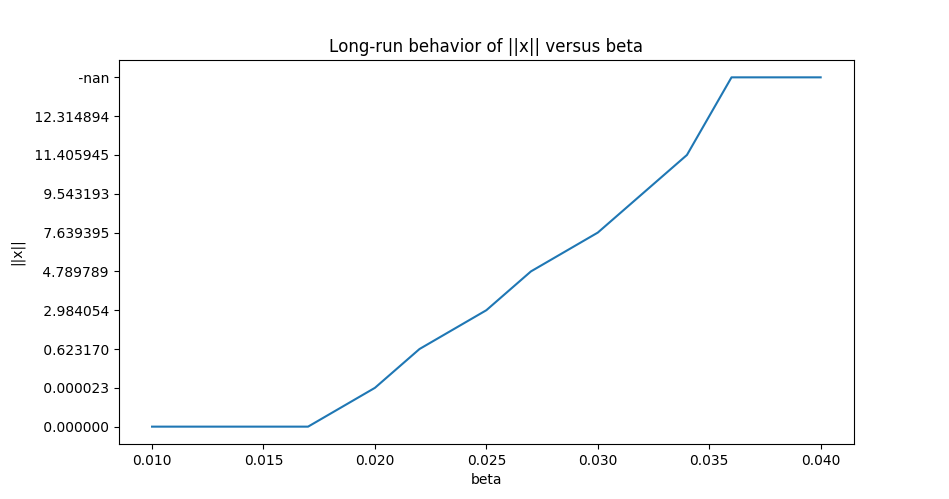
\includegraphics[scale=0.5]{hw4p4}
	\label{fig:hw4p4}
\end{figure}

\section*{Code (Ask Me For Precise Make/Run Instructions If Needed)}
\subsection*{Working C code}

	\begin{Verbatim}[xleftmargin=-5cm]
	static char help[] = "Homework 4 Problem 4 code\n\n";
	
	#include <petscts.h> //PETSc time steppers
	#include <petscsys.h>
	#include <petscmat.h>
	#include <mpi.h>
	#include <math.h>
	#include <stdbool.h>
	#include <stdlib.h>
	#include <limits.h>
	#include <float.h>
	#include <time.h>
	/**
	*
	* We're solving the system of ODEs 
	*
	* x' = beta * (1 - x) * Ax - gamma * x
	*
	* for scalars beta, gamma and adjacency matrix A.
	*/
	
	struct _n_prob_info
	{
	Mat A; /* adjacency matrix */
	Mat B;
	PetscReal beta, gamma; 
	PetscInt  n;
	/*bool print = true; print problem progress/info as it's being solved?*/
	
	/*	long int max_timesteps = 1E6;*/
	long int num_timesteps;
	PetscReal next_output; /*for adjoint stuff*/
	PetscReal tprev;
	/*	long int  N;problem size*/
	};
	
	/*problem context struct*/  
	typedef struct _n_prob_info *User;
	
	/*function that computes F(x,t) for system X' = F(X,t) */
	static PetscErrorCode RHSFunction(TS ts, PetscReal t, Vec X, Vec F, void* ctx)
	{
	PetscErrorCode     ierr;
	User               prob = (User)ctx;
	PetscScalar    	   *f;
	const PetscScalar  *x;
	PetscScalar 	   xval;
	PetscInt	   N, id;
	
	PetscFunctionBeginUser;
	
	ierr = MatMult(prob->B, X, F);CHKERRQ(ierr);
	ierr = VecScale(F, prob->beta);CHKERRQ(ierr);
	
	VecGetArrayRead(X, &x);
	VecGetArray(F, &f);
	VecGetLocalSize(F, &N);
	
	for(id = 0; id < N; ++id){
	xval = x[id];
	f[id] *= 1.0 - xval;
	f[id] -= prob->gamma * xval;
	}
	
	VecRestoreArrayRead(X, &x);
	VecRestoreArray(F, &f);
	
	PetscFunctionReturn(0);
	}
	
	
	static PetscErrorCode Monitor(TS ts, PetscInt step, PetscReal t, Vec X, void* ctx)
	{
	PetscErrorCode 		ierr;
	PetscReal 		dt, tprev;      
	User      		prob = (User)ctx; 
	
	TSGetTimeStep(ts, &dt);
	TSGetPrevTime(ts, &tprev);
	/*
	tsteps = prob->num_timesteps;
	
	if(tsteps == 0){
	// initial condition has not been set, error! 
	return(-1); //I should figure out what the appropriate PETSc error code here is, but this should never happen anyway...
	}
	else if(tsteps >= prob->max_timesteps - 1){
	//same
	return(-1);
	}
	prob->tprev = tprev;
	prob->t[tsteps] = tprev + dt;
	
	prob->xs[tsteps] = X;
	prob->num_timesteps++;
	*/
	PetscPrintf(PETSC_COMM_WORLD, "[%.1f] %D TS %.6f\n", (double)(prob->next_output), step, (double)t);
	return(0);
	}
	
	PetscErrorCode ApplyInitialConditions(Vec x, PetscScalar* initial_values)
	{
	/* NOTE: initial_values should contain ONLY the initial values
	* for the part of x owned by _this_ processor*/
	PetscScalar *x_ptr;
	PetscInt    N, id;
	/* I think you could also do this with VecSetValues(),
	* but I don't wanna get all the local indices and store them in a temp array*/
	VecGetArray(x, &x_ptr);
	VecGetLocalSize(x, &N);
	
	for(id = 0; id < N; ++id){
	x_ptr[id] = initial_values[id];
	}
	
	VecRestoreArray(x, &x_ptr);
	return(0);
	}
	
	static PetscErrorCode ApplyAdjointInitialConditions(Vec* lambda, int N)
	{
	PetscScalar *x_ptr;
	
	PetscInt id, rank, size, n_per_proc, remaining;
	
	MPI_Comm_size(PETSC_COMM_WORLD, &size);
	
	MPI_Comm_rank(PETSC_COMM_WORLD, &rank);
	
	n_per_proc = N/size;
	
	remaining = N % size;
	
	
	for(id = rank * n_per_proc; id < (rank+1)*n_per_proc; ++id){
	VecSet(lambda[id], 0.0);
	VecSetValue(lambda[id], id, 1.0, INSERT_VALUES);
	VecAssemblyBegin(lambda[id]);
	VecAssemblyEnd(lambda[id]);
	}
	
	/* handle rest of vectors*/
	for(id = n_per_proc * size; id < N; ++id){
	if(rank == id){
	VecSet(lambda[id], 0.0);
	VecSetValue(lambda[id], id, 1.0, INSERT_VALUES);
	VecAssemblyBegin(lambda[id]);
	VecAssemblyEnd(lambda[id]);
	}
	}
	
	return(0);
	}
	
	static PetscErrorCode ChungLuInvCDF(PetscReal p, PetscInt* k, PetscInt k0, PetscInt n, PetscReal gamma)
	{
	/* solves ChungLuCDF(k) = p */
	PetscReal cfactor, kc;
	
	cfactor = 1.0/(pow((PetscReal)k0, 1.0-gamma) - pow((PetscReal)n, 1.0-gamma));
	
	if(gamma > 1.0){
	kc = pow(p/cfactor, 1.0/(1.0 - gamma ));
	} else {
	
	kc = pow(p, 1.0/(1.0 - gamma)) / pow(cfactor, 1.0/(1.0 - gamma));
	}
	
	if(kc > n){
	kc = n;
	} 
	else if( kc < k0 ){
	kc = k0;
	}
	
	*k = round(kc);
	
	
	return(0);
	}
	
	static PetscErrorCode UniformSample(PetscReal *x, PetscReal low, PetscReal high)
	{
	*x = (double)rand() / nextafter((double)RAND_MAX, DBL_MAX);
	
	if(low != 0.0){
	*x += low;
	}
	if(high - low != 1.0){
	*x *= (high - low);
	}
	
	return(0);
	}
	
	
	static PetscErrorCode ChungLuSample(PetscInt* k, PetscInt k0, PetscInt n, PetscReal gamma)
	{
	/* returns a sample from the Chung-Lu distribution and places it in k */
	PetscErrorCode ierr;
	PetscReal      x;
	
	ierr = UniformSample(&x, 0.0, 1.0);
	
	ierr = ChungLuInvCDF(x, k, k0, n, gamma);
	
	return(0);
	}
	
	
	static PetscErrorCode RejectionChungLuSample(PetscBool* accepted, PetscInt candidate_kin,
	PetscInt candidate_kout, PetscReal kavg, PetscInt n)
	{
	PetscErrorCode ierr;
	PetscReal x,p, pnum, pdenom;
	
	/* no need to truncate p, since if p > 1 then the sample should always be accepted */
	
	pnum = (double)(candidate_kin * candidate_kout);
	pdenom = (double)(n * kavg) ;
	p = pnum/pdenom;
	/*
	PetscPrintf(PETSC_COMM_WORLD, "kavg = %f\n", kavg);
	PetscPrintf(PETSC_COMM_WORLD, "candkin = %f\n", candidate_kin);
	PetscPrintf(PETSC_COMM_WORLD, "candkout = %f\n", candidate_kout);
	PetscPrintf(PETSC_COMM_WORLD, "pn = %f\n", pnum);
	PetscPrintf(PETSC_COMM_WORLD, "pd = %f\n", pdenom);
	*/
	
	if(p >= 1.0){
	*accepted = true;
	return(0);
	}
	
	ierr = UniformSample(&x,0.0, 1.0);
	
	if(x < p){
	*accepted = true;
	} else {
	*accepted = false;
	}
	
	return ierr;
	}
	
	static PetscErrorCode SampleInfectedNodes(Vec prob_nodes_infected, PetscInt* count)
	{
	/* finds number of nodes that are infected and puts that into count */
	const PetscScalar* y;
	PetscScalar sampled_val;
	PetscInt N, id, n_infected;
	PetscErrorCode ierr;
	
	PetscFunctionBeginUser;
	VecGetArrayRead(prob_nodes_infected, &y);
	VecGetLocalSize(prob_nodes_infected, &N);
	
	n_infected = 0;
	
	for(id = 0; id < N; ++id){
	ierr = UniformSample(&sampled_val, 0.0, 1.0);
	if(y[id] > sampled_val){
	++n_infected;
	}
	}
	
	PetscFunctionReturn(ierr);
	}
	
	
	
	static PetscErrorCode 
	GenerateIIDCandidateChungLuDegreeDistributions(PetscInt* kin, PetscInt* kout, PetscReal* kavg, PetscInt n,
	PetscInt k0, PetscReal gamma)
	{
	srand(time(0));
	
	PetscInt ktotal, i, kcand;
	PetscErrorCode ierr;
	
	ktotal = 0;
	
	for(i = 0; i < n; ++i){
	/* do both samples in one iteration */
	ierr = ChungLuSample(&kcand, k0, n, gamma);
	kin[i] = kcand;
	ktotal += kcand;
	
	ierr = ChungLuSample(&kcand, k0, n, gamma);
	kout[i] = kcand;
	ktotal += kcand;
	}
	
	*kavg = (double)ktotal / (double)n;
	
	return(ierr);
	}
	
	
	
	
	
	static PetscErrorCode CreateAdjacencyMatrixCL(Mat* A, PetscInt k0, PetscInt n, PetscReal gamma, PetscBool write_to_file, char* filename)
	{
	PetscInt i, j, kin[n], kout[n], connected_list[n], count;
	
	PetscReal kavg;
	
	PetscBool accepted;
	
	PetscErrorCode ierr;
	
	
	ierr = GenerateIIDCandidateChungLuDegreeDistributions(kin, kout, &kavg, n, k0, gamma);
	/* really bad code segment cuz I don't have time */
	/*#ifdef WRITE_DD_CSV*/
	FILE* ddf;
	char targ_dd_buff[1024];
	snprintf(targ_dd_buff, sizeof(targ_dd_buff), "ChungLuTargetDDn%dk0%dg%f.csv", (int)n, (int)k0, (double)gamma);
	ddf = fopen(targ_dd_buff, "w");
	PetscFPrintf(PETSC_COMM_WORLD, ddf, "Target in-degree, Target out-degree\n");
	for(i = 0; i < n; ++i){
	PetscFPrintf(PETSC_COMM_WORLD, ddf, "%d, %d\n", kin[i], kout[i]);
	}
	fclose(ddf);
	/*#endif*/
	for(i = 0; i < n; ++i){
	count = 0;
	for(j = 0; j < n; ++j){
	ierr = RejectionChungLuSample(&accepted, kin[i], kout[j], kavg, n);
	if(accepted){
	connected_list[count] = j;
	++count;
	}
	}
	
	PetscInt index_list[count];
	PetscScalar	vals[count];
	/* copy into correctly-sized array for matrix insertion */
	for(j = 0; j < count; ++j){
	index_list[j] = connected_list[j];
	vals[j] = 1;
	}
	
	ierr = MatSetValues(*A, 1, &i, count, index_list, vals, INSERT_VALUES); CHKERRQ(ierr);
	}
	
	ierr = MatAssemblyBegin(*A, MAT_FINAL_ASSEMBLY);
	ierr = MatAssemblyEnd(*A, MAT_FINAL_ASSEMBLY);
	
	if(write_to_file){
	
	if(filename == NULL){
	memcpy(filename, "hw4mat.dat", sizeof("hw4mat.dat"));
	}
	
	PetscViewer viewer;
	ierr = PetscPrintf(PETSC_COMM_WORLD, "Writing matrix to binary file %s...\n", filename); CHKERRQ(ierr);
	ierr = PetscViewerBinaryOpen(PETSC_COMM_WORLD, filename, FILE_MODE_WRITE, &viewer);CHKERRQ(ierr);
	ierr = MatView(*A, viewer);CHKERRQ(ierr);
	}
	
	return(ierr);
	}
	
	static PetscErrorCode CreateAdjacencyMatrix(Mat A, PetscInt n, PetscInt* targ_kin, PetscInt* targ_kout, PetscBool write_to_file, char* filename)
	{
	PetscInt i, j, connected_list[n], count;
	
	PetscReal kavg;
	
	PetscBool accepted;
	
	PetscErrorCode ierr;
	PetscFunctionBeginUser;
	
	for(i = 0; i < n; ++i){
	kavg += 0.5 * (targ_kin[i] + targ_kout[i]);
	}
	
	kavg /= (PetscReal)n;
	
	for(i = 0; i < n; ++i){
	count = 0;
	for(j = 0; j < n; ++j){
	ierr = RejectionChungLuSample(&accepted, targ_kin[i], targ_kout[j], kavg, n);CHKERRQ(ierr);
	if(accepted){
	connected_list[count] = j;
	++count;
	}
	}
	
	PetscInt index_list[count];
	PetscScalar	vals[count];
	/* copy into correctly-sized array for matrix insertion */
	for(j = 0; j < count; ++j){
	index_list[j] = connected_list[j];
	vals[j] = 1;
	}
	
	ierr = MatSetValues(A, 1, &i, count, index_list, vals, INSERT_VALUES); CHKERRQ(ierr);
	}
	
	ierr = MatAssemblyBegin(A, MAT_FINAL_ASSEMBLY);
	ierr = MatAssemblyEnd(A, MAT_FINAL_ASSEMBLY);
	
	if(write_to_file){
	
	if(filename == NULL){
	memcpy(filename, "hw4mat.dat", sizeof("hw4mat.dat"));
	}
	
	PetscViewer viewer;
	ierr = PetscPrintf(PETSC_COMM_WORLD, "Writing matrix to binary file %s...\n", filename); CHKERRQ(ierr);
	ierr = PetscViewerBinaryOpen(PETSC_COMM_WORLD, filename, FILE_MODE_WRITE, &viewer);CHKERRQ(ierr);
	ierr = MatView(A, viewer);CHKERRQ(ierr);
	}
	
	PetscFunctionReturn(ierr);
	}
	
	static PetscErrorCode PowerLawInvCDF(PetscInt* k, PetscReal p,  PetscInt kmin, PetscReal alpha)
	{
	PetscFunctionBeginUser;
	*k = kmin * ((PetscInt)pow(1 - p, 1.0 / (1 - alpha)));
	PetscFunctionReturn(0);
	}
	
	static PetscErrorCode PowerLawIIDSample(PetscInt* ksamples, PetscInt n, PetscInt kmin, PetscReal alpha)
	{
	PetscFunctionBeginUser;
	PetscInt i, k;
	PetscErrorCode ierr;
	PetscReal p;
	for(i = 0; i < n; ++i){
	ierr = UniformSample(&p, 0.0, 1.0);
	ierr = PowerLawInvCDF(&k, p, kmin, alpha);CHKERRQ(ierr);
	ksamples[i] = k;
	}
	PetscFunctionReturn(ierr);
	}
	
	static PetscErrorCode UniformIntIIDSample(PetscInt* ksamples, PetscInt n, PetscInt low, PetscInt high)
	{
	PetscErrorCode ierr;
	PetscReal x;
	PetscInt i;
	PetscFunctionBeginUser;
	for(i = 0; i < n; ++i){
	ierr = UniformSample(&x, (double)low, (double)high);
	ksamples[i] = (PetscInt)(round(x));
	}
	PetscFunctionReturn(0);
	}
	
	
	static PetscErrorCode ReadPetscMatrix(const char filename[], Mat* readMat)
	{
	PetscErrorCode  ierr;
	PetscViewer     viewer;
	PetscFunctionBeginUser;
	
	ierr = PetscPrintf(PETSC_COMM_WORLD, "Reading in matrix from %s...\n",
	filename); CHKERRQ(ierr);
	ierr = PetscViewerBinaryOpen(PETSC_COMM_WORLD, filename,
	FILE_MODE_READ, &viewer); CHKERRQ(ierr);
	
	ierr = MatCreate(PETSC_COMM_WORLD, readMat); CHKERRQ(ierr);
	ierr = MatLoad(*readMat, viewer); CHKERRQ(ierr);
	ierr = PetscViewerDestroy(&viewer); CHKERRQ(ierr);
	
	ierr = PetscPrintf(PETSC_COMM_WORLD, "Successfully read matrix from %s.\n", filename); CHKERRQ(ierr);
	ierr = MatAssemblyBegin(*readMat, MAT_FINAL_ASSEMBLY);
	ierr = MatAssemblyEnd(*readMat, MAT_FINAL_ASSEMBLY);
	PetscFunctionReturn(ierr);
	}
	
	
	static PetscErrorCode Degree(Mat A, Vec k, Vec ones, const char* type)
	{
	PetscFunctionBeginUser;
	PetscErrorCode ierr;
	if(strcmp(type, "in") == 0){
	ierr = MatMultTranspose(A, ones, k);
	} else if(strcmp(type, "out") == 0){
	ierr = MatMult(A, ones, k);
	}
	PetscFunctionReturn(ierr);
	}
	
	static PetscErrorCode MeanDegree(Vec kin, PetscInt N, PetscReal* k)
	{
	PetscFunctionBeginUser;
	PetscErrorCode ierr;
	
	ierr = VecSum(kin, k);
	
	*k /= N;
	
	PetscFunctionReturn(ierr);
	}
	
	static PetscErrorCode MeanSquareDegree(Vec kin, PetscInt N, PetscReal* k)
	{
	PetscFunctionBeginUser;
	PetscErrorCode ierr;
	PetscReal x;
	ierr = VecNorm(kin, NORM_2, &x);
	*k = x * x / N;
	PetscFunctionReturn(ierr);
	}
	
	
	
	int main(int argc, char** argv)
	{
	TS             		ts; /* PETSc nonlinear solver/time-stepper*/            
	Vec            		x, kin, kout, ones, ones2;
	Mat            		J;   
	Mat            		Jp;
	PetscInt       		steps;
	PetscReal      		solve_time,xnorm, kmean, kinner, ksumsq, time_length = 100.0;
	PetscReal               step_size=0.1;
	PetscBool      		flag, wflag, monitor = PETSC_FALSE, read_mat = PETSC_FALSE, write_mat = PETSC_TRUE;
	char                    filename[100], writefile[100];
	FILE                    *wf;
	PetscMPIInt    		size, rank;
	/*Vec                     *lambda, *mu;adjoint variables*/
	struct _n_prob_info 	user;
	/*KSP			ksp;Krylov solver for eigenvalues of A*/
	PetscErrorCode          ierr=0;
	
	PetscInitialize(&argc, &argv, NULL, help);if(ierr) return ierr;
	
	MPI_Comm_size(PETSC_COMM_WORLD, &size);
	
	MPI_Comm_rank(PETSC_COMM_WORLD, &rank);
	
	if(rank == 0){
	PetscPrintf(PETSC_COMM_WORLD, "Program initialized with %d processes.\n", size);
	}
	
	PetscOptionsGetReal(NULL, NULL, "-beta", &user.beta, &flag);
	/*PetscOptionsGetInt(NULL, NULL, "-k0", &user.k0, &flag);*/
	PetscOptionsGetInt(NULL, NULL, "-n", &user.n, &flag);
	if(!flag){
	PetscOptionsGetInt(NULL, NULL, "-N", &user.n, &flag);
	}
	PetscOptionsGetReal(NULL, NULL, "-g", &user.gamma, &flag);
	if(!flag){
	PetscOptionsGetReal(NULL, NULL, "--gamma", &user.gamma, &flag);
	}
	PetscOptionsGetBool(NULL, NULL, "-m",&monitor, &flag);
	if(!flag){
	PetscOptionsGetBool(NULL, NULL, "--monitor",&monitor, &flag);
	}
	PetscOptionsGetBool(NULL, NULL, "-r",&read_mat, &flag);
	if(!flag){
	PetscOptionsGetBool(NULL, NULL, "--read",&read_mat, &flag);
	}
	PetscOptionsGetBool(NULL, NULL, "-w",&write_mat, &flag);
	if(!flag){
	PetscOptionsGetBool(NULL, NULL, "--write",&write_mat, &flag);
	}
	PetscOptionsGetString(NULL, NULL, "-wfl", writefile, 100, &wflag);
	if(!wflag){
	PetscOptionsGetString(NULL, NULL, "--writefile",writefile, 100, &wflag); /* 100 is max length of filename in characters, including null-terminator*/
	}
	
	
	PetscOptionsGetString(NULL, NULL, "-f",filename, 100, &flag); /* 100 is max length of filename in characters, including null-terminator*/
	if(!flag){
	PetscOptionsGetString(NULL, NULL, "--filename",filename, 100, &flag); /* 100 is max length of filename in characters, including null-terminator*/
	}
	if(rank == 0){
	ierr = PetscPrintf(PETSC_COMM_WORLD, "Options set. Getting matrices.\n");
	}
	
	user.num_timesteps = 0;
	
	/*create matrices and vectors*/
	MatCreate(PETSC_COMM_WORLD, &user.A);
	MatSetSizes(user.A, PETSC_DECIDE, PETSC_DECIDE, user.n, user.n);
	MatSetUp(user.A);
	
	MatCreate(PETSC_COMM_WORLD, &user.B);
	MatSetSizes(user.B, PETSC_DECIDE, PETSC_DECIDE, user.n, user.n);
	MatSetUp(user.B);
	
	if(read_mat){
	ierr = ReadPetscMatrix(filename, &user.B); CHKERRQ(ierr);
	
	} else {
	PetscInt targ_k[user.n];
	PetscReal alpha = 4.0;
	PetscInt kmin = 50, kunifmax = 100;
	ierr = PowerLawIIDSample(targ_k, user.n, kmin, alpha);
	ierr = CreateAdjacencyMatrix(user.B, user.n, targ_k, targ_k, true, "hw4plmat.dat");
	/*ierr = UniformIntIIDSample(targ_k, user.n, kmin, kunifmax);
	ierr = CreateAdjacencyMatrix(user.A, user.n, targ_k, targ_k, true, "hw4unifmat.dat");*/
	}
	
	MatCreate(PETSC_COMM_WORLD, &J);
	MatSetSizes(J, PETSC_DECIDE, PETSC_DECIDE, user.n, user.n);
	MatSetUp(J);
	MatCreateVecs(J, &x, NULL); /*sets up the vectors x in a parallel format that plays nicely with the Jacobian)*/
	
	MatCreate(PETSC_COMM_WORLD, &Jp);
	MatSetSizes(Jp, PETSC_DECIDE, PETSC_DECIDE, user.n, 1);
	MatSetUp(Jp);
	
	VecCreateMPI(PETSC_COMM_WORLD, PETSC_DECIDE, user.n, &ones);
	VecSet(ones, 1.0);
	
	VecCreateMPI(PETSC_COMM_WORLD, PETSC_DECIDE, user.n, &kin);
	VecCreateMPI(PETSC_COMM_WORLD, PETSC_DECIDE, user.n, &kout);
	VecCreateMPI(PETSC_COMM_WORLD, PETSC_DECIDE, user.n, &ones2);
	
	
	/*
	
	ierr = Degree(user.A, kin, ones, "in");
	
	ierr = Degree(user.A, kout, ones, "out");
	
	ierr = MeanDegree(kin, user.n, &kmean);CHKERRQ(ierr);
	
	ierr = VecDot(kin, kout, &kinner);
	
	kinner /= user.n;
	
	ierr = MeanSquareDegree(kin, user.n, &ksumsq);
	
	PetscPrintf(PETSC_COMM_WORLD, "For the matrix with uniformly-distributed target degree distribution: \n <kin, kout> = %f,\n <k> = %f, \n <kin,kout>/<k> = %f,\n <k^2> = %f.\n", kinner, kmean, kinner/kmean, ksumsq);
	*/
	ierr = Degree(user.B, kin, ones, "in");
	
	ierr = Degree(user.B, kout, ones, "out");
	
	ierr = MeanDegree(kin, user.n, &kmean);CHKERRQ(ierr);
	
	ierr = VecDot(kin, kout, &kinner);
	
	kinner /= user.n;
	
	ierr = MeanSquareDegree(kin, user.n, &ksumsq);
	
	PetscPrintf(PETSC_COMM_WORLD, "For the matrix with power law-distributed target degree distribution: \n <kin, kout> = %f,\n <k> = %f, \n <kin,kout>/<k> = %f,\n <k^2> = %f.\n", kinner, kmean, kinner/kmean, ksumsq);
	
	/*ierr = KSPCreate(PETSC_COMM_WORLD, &ksp);
	ierr = KSPSetFromOptions(ksp);CHKERRQ(ierr);*/
	
	/*power method for eigenvalues 'cuz who really cares about speed? (says the guy writing this big 'ol C file...)*/
	PetscInt i;
	/*
	for(i = 0; i < 100; ++i){
	ierr = MatMult(user.A, ones, ones2);
	ierr = VecCopy(ones2, ones);
	}
	
	VecNorm(ones2, NORM_2, &xnorm);
	
	xnorm = pow(xnorm, 1.0/100.0);
	
	PetscPrintf(PETSC_COMM_WORLD, "Largest eigenvalue (uniform network): %f\n", xnorm);
	*/
	VecSet(ones, 1.0);
	VecSet(ones2, 1.0);
	for(i = 0; i < 20; ++i){
	ierr = MatMult(user.B, ones, ones2);
	ierr = VecCopy(ones2, ones);
	}
	
	VecNorm(ones2, NORM_2, &xnorm);
	
	xnorm = pow(xnorm, 1.0/20.0);
	
	PetscPrintf(PETSC_COMM_WORLD, "Largest eigenvalue (power law network): %f\n", xnorm);
	
	/* create TS context */
	TSCreate(PETSC_COMM_WORLD, &ts);
	TSSetFromOptions(ts);
	TSSetMaxTime(ts, time_length);
	TSSetRHSFunction(ts, NULL, RHSFunction, &user);
	TSSetTimeStep(ts, step_size);
	
	/* set Jacobian for adjoint problem */
	/*TSSetRHSJacobian(ts, J, J, RHSJacobian, &user);*/
	
	TSSetExactFinalTime(ts, TS_EXACTFINALTIME_INTERPOLATE); /* if the TS goes over the allotted time_length, interpolate back to it*/
	TSSetProblemType(ts, TS_NONLINEAR);
	
	/*TSSetSaveTrajectory(ts);*/
	
	if(monitor){
	TSMonitorSet(ts, Monitor, &user, NULL);
	}
	
	/* TODO: apply random initial conditions to x */
	PetscReal ic[user.n];
	for(i = 0; i < user.n; ++i){
	UniformSample(&ic[i], 0.0, 0.1);
	}
	
	ApplyInitialConditions(x, ic);
	
	/* solve the forward model */
	TSSolve(ts, x);
	TSGetSolveTime(ts, &solve_time);
	TSGetStepNumber(ts, &steps);
	
	PetscPrintf(PETSC_COMM_WORLD, "Solver took %D steps, completed solve in time %d\n", steps, (double)solve_time);
	
	VecNorm(x, NORM_2, &xnorm);
	/* TODO: adjoint solve */
	
	
	
	PetscPrintf(PETSC_COMM_WORLD, "||x|| = %f\n", xnorm);
	
	if(wflag){
	wf = fopen(writefile, "a");
	ierr = PetscFPrintf(PETSC_COMM_WORLD, wf, "beta, %f, ||x||, %f\n", user.beta, xnorm);
	ierr = fclose(wf);
	}
	
	/* cleanup */
	MatDestroy(&J);
	MatDestroy(&Jp);
	VecDestroy(&x);
	TSDestroy(&ts);
	
	PetscFinalize();
	return ierr;
	}
	
	\end{Verbatim}
	
	\subsection*{Python Code}
	\begin{Verbatim}
	import matplotlib.pyplot as plt
	import pandas as pd
	
	if __name__ == '__main__':
	
	dat = pd.read_csv("hw4res.csv").to_numpy()
	
	plt.figure()
	plt.plot(dat[:,0], dat[:,1])
	plt.xlabel("beta")
	plt.ylabel("||x||")
	plt.title("Long-run behavior of ||x|| versus beta")
	plt.show()
	\end{Verbatim}
\end{document}